\documentclass{article}
\usepackage{neurips_2026}
\usepackage[utf8]{inputenc}
\usepackage[T1]{fontenc}
\usepackage{courier}
\usepackage{hyperref}
\usepackage{url}
\usepackage{booktabs,array}
\usepackage{amsmath,amssymb,amsthm,amsfonts}
\usepackage{graphicx}
\usepackage{microtype}
\usepackage[table]{xcolor}
\usepackage[capitalise]{cleveref}

\newtheorem{proposition}{Proposition}

\title{What Does It Cost to Buy First Place? Targeted Investment, Aggregation Rules, and the Breadth--Depth Price of a Multi-Task Leaderboard}
\author{Anonymous Author(s)}

\begin{document}
\maketitle

\begin{abstract}
Multi-task leaderboards compress many task scores into one ranking, and a developer can raise a target model on chosen tasks by training on related data. We ask what first place must cost under each aggregation rule. We define the price of first place by its breadth (tasks touched), its depth (total boost) and its feasibility under a per-task boost budget, solve it for six rule families (exactly, or with a reported optimality gap), and measure it for the 30 highest-ranked models on HELM MMLU (57 subjects) and on the Open LLM Leaderboard at benchmark level (6 tasks) and sub-task level (39 tasks), where the number of tasks varies on the same models. At ceilings and in points the mean family is the dearest rule on every board, by a factor of 7 to 19 over the cheapest (a median over targets of 360 points against 19 for plurality on HELM), but which rule is cheapest depends on the board, and no rule is cheapest for 90\% of targets on any board. Our pre-registered expectation that median and majority rules need more breadth than the mean is reversed on HELM and holds only in part on the Open LLM Leaderboard, and the effect of the number of tasks differs by rule and changes sign with the budget. Under score noise, holding first place with 90\% confidence costs the median rule and the minimum 3 to 7 times their noise-free depth, against 1.2 to 2 times for the mean family. Within a board the gap to the incumbent predicts the price of most rules, but the fitted relation fails to transfer between boards in at least one direction for every rule (for the mean, only through the number of tasks), and summaries of the deficit profile add little to it.
\end{abstract}

\section{Introduction}
\label{sec:intro}

Public leaderboards turn many task scores into one ranking, and the ranking decides which model is called best. HELM \citep{liang2022helm} and the Open LLM Leaderboard rank models over many tasks by an aggregate score. A developer who wants a model to be first can train it on data related to some of the tasks, and there is evidence that models are in practice trained on or tuned to benchmark data \citep{zhou2023cheater,yang2023rephrased,singh2025illusion}. What does first place then cost, and does the answer depend on how the board aggregates?

The cost has two coordinates. \emph{Breadth} is the number of tasks the developer must work on; \emph{depth} is the total improvement they must buy. A budget on the improvement of a single task limits both. A common intuition, borrowed from robust statistics, is that rules which need a majority of tasks (medians, plurality) are harder to buy than an average because they demand breadth. Whether this holds for a finite margin of victory on real leaderboards, how large the differences between rules are, and how the answer changes when the same models are scored on fewer, coarser tasks or on more, finer ones, is not known.

\begin{figure}[t]
\centering
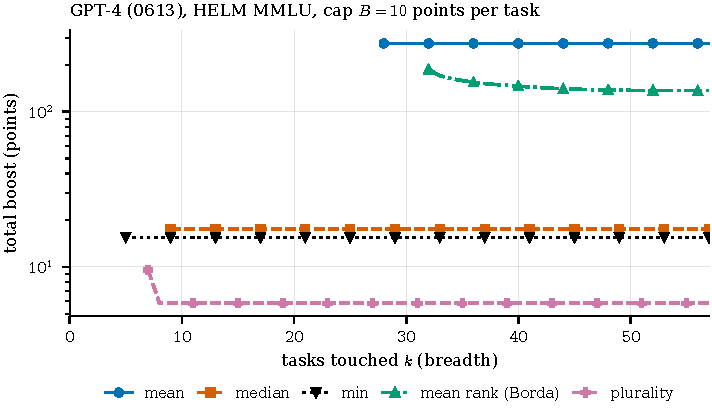
\includegraphics{../figures/fig1_teaser.pdf}
\caption{Different rules make different plans cheapest: least total boost (log scale) against tasks touched, for one target (GPT-4 0613, the one with the median range of minimal breadth across rules) on HELM MMLU at a cap of 10 points per task and each rule's own leader. The mean needs far more total boost than the median, minimum and plurality, and cannot be bought with fewer than about 28 tasks at this cap.}
\label{fig:teaser}
\end{figure}

We measure it. We define the price of first place as the breadth, depth and feasibility of the cheapest plan that puts a target model first under a rule, solve it exactly for six rule families, and compute it for the top-ranked models of three public boards: the 57 MMLU subjects of HELM and the Open LLM Leaderboard at benchmark level (six tasks) and at sub-task level (39 tasks), the latter two on the same models. We state in advance which outcomes would refute our expectations; two of them occur. Three results follow.
\begin{itemize}
\item \emph{The rules' prices differ by a factor of 7 to 19 in total boost, and the cheapest rule differs by board.} At ceilings and in the board's own points, the median over targets not yet first puts a target first on HELM for 360 points under the mean, against 36 under the median rule and 19 under plurality; on the Open LLM Leaderboard the mean needs 32 and 134 points at benchmark and sub-task level against 5 and 10 for the median rule. That the mean is dearest in points is close to an identity (its price is the sum of the deficits); the content is the size of the spread, which varies with caps and units.
\item \emph{The expected breadth ordering fails.} Median and majority rules need less breadth than the mean on HELM, the reverse of our prediction, and hold the predicted order only in part on the Open LLM Leaderboard. The dependence on the number of tasks is rule-specific and changes sign with the budget, so task granularity has no uniformly safe direction, and no rule is cheapest for 90\% of the targets on any board.
\item \emph{Cheap first place is fragile.} Holding first place with 90\% confidence under score noise costs the median rule and the minimum 3 to 7 times their noise-free depth, against 1.2 to 2 times for the mean family, on HELM and on the sub-task board.
\end{itemize}

\paragraph{Contributions.}
(i) The price of first place as a breadth--depth--feasibility triple under a boost budget, with exact solutions per rule class, computed on three public boards, with solvers checked against exhaustive search and an optimality gap reported where it is not zero (\Cref{sec:setting,sec:exact}). (ii) Pre-registered predictions reported with the verdicts as they came out: the breakdown-point intuition fails for a finite margin, and the ordering of the rules depends on the board, budget, cap and unit (\Cref{sec:breadth}). (iii) Quantities a designer can use: the budget at which the breadth ordering of two rule classes crosses, price magnitudes per rule, a within-board relation between gap and price that does not transfer across boards, and the price of confident first place under noise (\Cref{sec:pricemap,sec:predictors,sec:robustness}). A hypothesis that deficit-profile summaries predict price beyond the gap was tested and mostly failed. (iv) A calibration of the boost scale, where the conclusions hold and do not (\Cref{sec:discussion}), and a released package that prices first place on any score matrix under the seven rules studied; code and result tables are released with the paper.

\section{Related Work}
\label{sec:related}

\paragraph{Sensitivity and diversity of multi-task rankings.}
\citet{zhang2024diversity} treat a multi-task benchmark as a social-choice problem, separate cardinal from ordinal aggregation, and show a trade-off between the diversity of a benchmark and the stability of its ranking when noise is injected into tasks. That perturbation is untargeted. We ask what a developer who \emph{chooses} the tasks must spend to put one given model first, and use their cardinal/ordinal taxonomy and the dispersion and correlation of task scores as candidate predictors of the price (\Cref{sec:predictors}). Finite-sample robustness metrics ask how little data must change to flip a conclusion \citep{broderick2020dropping}; ours is the smallest change to one model's scores that flips a leaderboard.

\paragraph{Strategic post-training and contamination.}
\citet{chen2026incentives} model a designer and several developers who each choose a scalar benchmark-specific effort; their benchmark has one score, so the aggregation across tasks, our subject, is absent, and their results are theoretical. We give the single-developer, multi-task measurement on real leaderboards. \citet{dominguez2024testtask} discuss training on data related to the evaluation tasks as a confound, and \citet{zhang2025trainbeforetest} propose giving every model the same task-specific fine-tuning before testing; we cite both for the mechanism. Private testing on Chatbot Arena \citep{singh2025illusion}, benchmark data in training \citep{zhou2023cheater} and rephrased test samples \citep{yang2023rephrased} show that the actions we price occur; they do not measure a price per aggregation rule.

\paragraph{Aggregation rules and social choice.}
Voting rules have been applied to rank agents and models over tasks \citep{lanctot2023social,rofin2023votenrank}, Nash averaging makes the ranking invariant to redundant tasks and models \citep{balduzzi2018reevaluating}, and the choice of tasks can itself reorder methods \citep{dehghani2021lottery}; these works compare rules by axioms or ranking agreement, not by the cost of moving one model to the top. Our price is a cardinal bribery problem with ceilings \citep{brandt2016comsoc,bredereck2016shift}, and the intuition from robust statistics is that a rule with a high breakdown point, such as the median, is expensive to capture. For a finite margin of victory the price is instead a function of the target's deficits, and the intuition has the wrong sign on HELM and depends on board and budget elsewhere (\Cref{sec:pricemap,sec:breadth}).

\section{Setting: the price of first place}
\label{sec:setting}

\paragraph{Leaderboard and aggregation.}
A leaderboard is a score matrix $S\in\mathbb{R}^{N\times m}$ of $N$ models on $m$ tasks, each task $j$ with a ceiling $c_j$ (e.g.\ 100 points). An aggregation rule $A$ maps the matrix to a score or a ranking of the models. We study six rule groups: the mean (raw, and its $z$-scored, geometric and $p$-mean variants as one family), the median and other quantiles, the minimum, the mean rank (Borda), which with ties counted as half is the mean win rate, the plurality of task wins, and Copeland's pairwise-majority score.

\paragraph{Targeted investment.}
A developer picks a target model $t$ and a boost $\delta\in\mathbb{R}^m_{\ge 0}$; the target's score on task $j$ becomes $\min(S_{tj}+\delta_j,\,c_j)$ and every other score is unchanged. The boost stands for training on data related to the task; we train nothing, a boost is the \emph{input} whose cost we measure, and \Cref{sec:calibration} checks its scale against observed fine-tunes. The developer is static and acts once, rivals do not respond, and boosts on different tasks do not interact (\Cref{sec:discussion}). Per-task boosts are capped by a \emph{boost budget} $B$: $\delta_j\le B$. We report price as a function of $B$ and the smallest feasible budget $B^\ast_A(t)$ at which first place under rule $A$ is attainable. ``First'' means ahead of every rival by a margin $\varepsilon>0$ (ties lose).

\paragraph{Price: breadth, depth, feasibility.}
The investment has two coordinates. Its \emph{breadth} is the number of tasks touched, $k=\lVert\delta\rVert_0$, and its \emph{depth} is the total boost $\lVert\delta\rVert_1$, measured in points of the board's own scale (robustness: in standard deviations of the task, as a fraction of headroom, and under a convex cost; \Cref{sec:robustness}). The \emph{breadth--depth frontier} $C_A(k)$ is the least depth of a plan that makes $t$ first under $A$ using at most $k$ tasks; it is infinite where no plan is feasible under $B$ and the ceilings. The \emph{targeting multiplier} is the depth of the cheapest untargeted plan (the same boost on every task) divided by the depth of the cheapest targeted plan. Across boards with different $m$ we use the breadth fraction $k/m$, the per-task depth $\lVert\delta\rVert_1/m$ and $B$ in task standard deviations.

\paragraph{Incumbents.}
Rules crown different leaders, so a lower price under one rule can mean only that its leader is weaker. We therefore report the price against each rule's own leader and against a common incumbent set, the top models under the board's official rule.

\section{The exact price by rule class}
\label{sec:exact}

The six rule groups fall into four classes by how a boost on one task moves the target's standing (\Cref{tab:rules}). Within a class the cheapest plan has a closed form or a small exact program; this lets us report optima, not a heuristic's, on boards with thousands of models. For rules whose rival scores do not depend on the target (mean family, quantiles), let $V=\max_{i\ne t}A_i(S)+\varepsilon$ be the level the target's aggregate must reach, and $d_j=V-S_{tj}$ the shortfall on task $j$ in the case of a quantile rule. Costs are linear in points unless stated.

\begin{table}[t]
\caption{Rule classes, what a boost buys, and the price each class implies. $a$ is the number of tasks on which the target already scores at least the rival level $V$, $r$ the rank of the order statistic ($r=m$ for the minimum, $r=\lceil m/2\rceil$ for the median), $G$ the aggregate gap, $u_j=\min(B,c_j-S_{tj})$ the headroom on task $j$.}
\label{tab:rules}
\centering\small
\begin{tabular}{@{}p{2.3cm}p{2.7cm}p{3.1cm}p{3.0cm}@{}}
\toprule
Rule & Influence of a boost & Minimal breadth & Depth at that breadth\\
\midrule
Mean family & linear, capped by headroom & fewest tasks whose headroom $\sum w_ju_j$ covers $G$ & fixed: $mG$ (raw mean), however spread\\
Quantile, median, min & none beyond level $V$ & $\max(0,r-a)$ & the $r-a$ smallest shortfalls $d_j$\\
Mean rank (= mean win rate) & steps, bounded per task & at least $\lceil g/N\rceil$ for deficit $g$ & optimum of a covering program (levels per task)\\
Plurality, Copeland & steps, coupled across tasks & optimum of an integer program & its optimum\\
\bottomrule
\end{tabular}
\end{table}

\begin{proposition}[Quantile rules]\label{prop:quantile}
Let $A$ be the $r$-th largest task score. The target needs at least $r$ tasks at level $V$ or above, so its minimal breadth is $\max(0,r-a)$. The cheapest plan with that breadth raises the $r-a$ tasks of smallest shortfall exactly to $V$; it is feasible under budget $B$ if and only if the $(r-a)$-th smallest shortfall is at most $B$ (and at most the task's headroom). Any boost beyond $V$ on a task, and any additional task, adds depth and removes nothing from the price.
\end{proposition}

\begin{proposition}[Mean family]\label{prop:mean}
Let $A_i=\sum_j w_jS_{ij}$ with weights $w_j>0$ (raw mean: $w_j=1/m$; $z$-scored mean: $w_j=1/(m\sigma_j)$) and gap $G=V-A_t>0$. First place is feasible under $B$ if and only if $\sum_jw_ju_j\ge G$. Under a linear cost $\sum_j\kappa_j\delta_j$ the optimum fills tasks in decreasing order of $w_j/\kappa_j$; for the raw mean in points the depth is $mG$ however it is spread over tasks. The minimal breadth is the least $k$ for which the $k$ largest $w_ju_j$ sum to at least $G$. Only under a scaled or convex cost does the allocation change the depth, and then it is water-filling.
\end{proposition}

\begin{proposition}[Additive rank rules]\label{prop:rank}
Under mean rank (Borda; with ties counted as half it equals the mean win rate) the margin of the target over a fixed rival $i$ is a sum over tasks of non-decreasing step functions of $\delta_j$, with at most $N-1$ steps per task (one for each model passed). The price is therefore the optimum of a multiple-choice covering problem with one constraint for each rival, and a boost beyond the best rival's score on a task buys nothing. In pairwise-win units each task can raise the margin over $i$ by at most $N$, so the breadth is at least $\lceil g_i/N\rceil$ for a deficit $g_i$.
\end{proposition}

\begin{proposition}[Coupled rules]\label{prop:coupled}
Under plurality the target wins a task only by passing the best rival there, and each such win also removes one win from that rival; under Copeland the target beats a rival only if it passes them on more tasks than they pass it. In both cases the effect of boosting a task depends on which other tasks are boosted, and the price is an integer program with one constraint per rival.
\end{proposition}

Proofs are in \Cref{app:proofs}.

\paragraph{Solvers and checks.}
We compute the optimum for the quantile and mean classes in closed form, and for the rank and coupled classes with mixed-integer programs (HiGHS) over the per-task levels, with rival constraints added lazily where a rule has one per rival; each plan returned is re-evaluated and is first under the rule on every price we report. Every solver agreed with exhaustive enumeration of integer plans on random instances of at most 7 models and 5 tasks (4 for the rank and coupled rules) (217 to 2072 instances per rule, all agreeing). Plurality is solved to optimality on every board. The mean rank and Copeland programs are solved to a reported optimality gap, which is zero at benchmark level and for the top-30 HELM targets at ceilings and up to 12\% (Borda) and 7\% (Copeland) on the top-30 sub-task targets; where it is not zero the price is an upper bound (\Cref{tab:price}).

\paragraph{No rule is cheapest everywhere.}
The classes give no universal ordering: with two models and three tasks, the target $(59,59,0)$ against a rival $(60,60,60)$ needs about 2 points under the median but about 62 under the mean (\Cref{app:proofs}). Whether and where this matters on real boards is the question of \Cref{sec:results}.

\section{Data and protocol}
\label{sec:data}

\paragraph{Boards.}
We use three public regimes, all frozen snapshots. \emph{HELM MMLU} (release v1.13.0) gives the accuracy of $N=79$ models on the $m=57$ MMLU subjects~\citep{hendrycks2021mmlu,liang2022helm}. The \emph{Open LLM Leaderboard}~\citep{fourrier2024olb}, which runs the Evaluation Harness~\citep{gao2023harness}, in the frozen snapshot of its \texttt{contents} table, gives each model's score on six benchmarks (IFEval, BBH, MATH, GPQA, MuSR, MMLU-Pro~\citep{zhou2023ifeval,suzgun2022bbh,hendrycks2021math,rein2023gpqa,sprague2023musr,wang2024mmlupro}; $m=6$, each normalised by the board from its chance level to 100); its \texttt{results} snapshot gives, for the same models, the scores on $m=39$ sub-tasks (24 BBH, 3 GPQA, 7 MATH and 3 MuSR tasks, MMLU-Pro and IFEval as single tasks) with standard errors, so that the same models can be priced at $m=6$ and at $m=39$. The benchmark-level board has $N=2179$ models and the sub-task board $N=2083$ (the models of the \texttt{results} snapshot that match a \texttt{contents} row). Noise is binomial on HELM, the reported standard error on the sub-task board, and absent in \texttt{contents}.


\paragraph{Targets, incumbents, slices.}
The targets are the 30 models ranked highest by the board's official rule on each board. Merged, flagged and not-on-hub models are excluded as targets and incumbents, since the top of the board is a crowded family of derivatives of a few bases.

\paragraph{Boost budgets and units.}
The grid of boost budgets is $B\in\{2,5,10,20\}$ points and its equivalent in task standard deviations, fixed in advance. \Cref{sec:calibration} says which end of it observed fine-tunes make plausible. The primary unit of investment is points on the board's scale; the other three are standard deviations $\sigma_j$ computed once on the full board of each granularity, the fraction of headroom, and a convex cost $\sum_j(\delta_j/\sigma_j)^\gamma$ with $\gamma\in\{1,2\}$.

\paragraph{Varying $m$ on the same models.}
To separate the number of tasks from the number of models, we draw on HELM random subsets of $m\in\{5,\dots,57\}$ subjects, paired across rules, and on the Open LLM Leaderboard price the same models with \emph{bundled} plans (a benchmark-level boost lifts all of the benchmark's sub-tasks together) and \emph{free} plans (each sub-task boosted separately; bundled plans are a subset, so the free price is the lower). Across $m$ we compare breadth fractions and $B$ in standard deviations of the granularity analysed.

\paragraph{Uncertainty.}
Targets that share an incumbent or a model family are not independent. All intervals on comparisons across targets are cluster bootstrap intervals, resampling incumbents and families (the resolved base model or organisation on the Open LLM Leaderboard, the organisation on HELM); on HELM random subsets the draws are paired across rules.

\paragraph{Pre-registered tests.}
The following thresholds were fixed in advance of the results; the verdicts we report in \Cref{sec:results} follow them whatever their direction.
\begin{description}
\item[R1 (breadth).] At $m=57$ on HELM and $m=39$ on the Open LLM Leaderboard (free plans; pre-registered as $m\approx45$, which the data do not provide), median, plurality and Copeland (the ``median-type'' rules) need strictly more breadth $k/m$ than the mean family, at $B$ equal to the median $B^\ast$ of the mean family or larger, for a share $p$ of the top-30 targets. \emph{Supported} if $p\ge80\%$ and the paired-difference interval excludes 0; \emph{partially supported} if $60\%\le p<80\%$ and it excludes 0; \emph{failed} if $p<60\%$ or the interval contains 0.
\item[R2 (no dominance).] Refuted if one rule has the lowest depth at fixed $B$ for at least 90\% of targets on every board.
\item[R3 (gap insufficiency).] The prediction is that the gap alone is not sufficient: within a rule, across targets, the rule-specific gap to the incumbent (the aggregate difference on the rule's own scale; the rank-score or win-rate difference for Borda; the deficit in task wins or pairwise wins for plurality and Copeland) is fitted on one board to the log depth at fixed $B$ and evaluated on another in each of the six directions (we report the worst and the best). The prediction is refuted for a rule only if the held-out $R^2$ is at least $0.9$ in every direction (lower interval limit of the worst direction); it is supported if the gap fails in at least one. The test concerns transfer across boards; it does not say that price is unpredictable.
\item[R4 (the $m$-effect).] The ratio of breadth fractions (median-type over the mean family) rises with $m$; refuted if the cluster-bootstrap interval of its slope over $m$ includes 0. Reported separately for free and bundled plans.
\item[R5 (units).] The median-type rules lie on the same side of the mean family in all four units (cheaper, as predicted), with a minimum Kendall $\tau\ge0.5$ between the rule orderings; otherwise the ordering is reported as unit-dependent.
\end{description}

\section{Results}
\label{sec:results}

Prices are for the 30 highest-ranked targets of each board against each rule's own leader unless stated, with cluster-bootstrap intervals (\Cref{sec:data}). ``Ceilings'' means the per-task boost is limited only by the task ceiling ($B\to\infty$).

\subsection{The price map: total boost is where the rules differ most}
\label{sec:pricemap}

\Cref{tab:price} gives the price of first place for each rule and board. With boosts limited only by ceilings, first place is feasible for every target under every rule, and the boost needed differs by a factor of 7 to 19 between the mean and the cheapest rule on each board. We report medians over the targets that are not already first under the rule (at most two per board and rule), because the others price at zero. The mean family is the expensive one: on HELM the median total boost is 360 points for the mean against 19 for plurality, 26 for the minimum and 36 for the median rule; on the Open LLM Leaderboard at sub-task level 134 against 10 for the median rule and 82 for plurality; at benchmark level 32 against 5 to 23 for the other rules. This follows \Cref{prop:mean}: the total boost under a mean is $m$ times the gap however it is spread, whereas the order and majority rules need a level on some tasks and nothing more. The mean's breadth is small: at ceilings it closes its gap on a median of 16\% of the HELM subjects, against two thirds for Copeland.

Targeting pays most for the rules that reward it (\Cref{fig:map}, Appendix~\ref{app:figs}): on HELM the depth of the cheapest uniform plan over that of the cheapest targeted plan is 1 for the mean by construction and 9 to 20 for plurality, median and minimum.

\begin{table}[t]
\centering
\caption{Price of first place at ceilings (medians over the 30 highest-ranked targets not yet first, own leader): total boost in points, breadth fraction $k/m$ and minimal feasible per-task budget $B^\ast$ in points. $\dagger$: some solver runs did not close (gap above $10^{-4}$); the cell is an upper bound.}
\label{tab:price}
\footnotesize\setlength{\tabcolsep}{3.5pt}
\begin{tabular}{@{}lrrrrrrrrr@{}}
\toprule
 & \multicolumn{3}{c}{HELM MMLU ($m{=}57$)} & \multicolumn{3}{c}{OLLB benchmarks ($m{=}6$)} & \multicolumn{3}{c}{OLLB sub-tasks ($m{=}39$)}\\
\cmidrule(lr){2-4}\cmidrule(lr){5-7}\cmidrule(lr){8-10}
Rule & boost & $k/m$ & $B^\ast$ & boost & $k/m$ & $B^\ast$ & boost & $k/m$ & $B^\ast$\\
\midrule
mean & 360 & 0.16 & 6.5 & 32 & 0.17 & 5.3 & 134 & 0.05 & 3.5\\
z-mean & 223 & 0.12 & 5.8 & 23 & 0.17 & 7.3 & 111 & 0.05 & 7.2\\
median & 36 & 0.20 & 4.9 & 5 & 0.17 & 2.4 & 10 & 0.13 & 5.1\\
min & 26 & 0.09 & 11.5 & 8 & 0.33 & 5.1 & 20 & 0.08 & 9.9\\
Borda & 222 & 0.58 & 6.0 & 9 & 0.17 & 3.6 & 26$^\dagger$ & 0.10 & 2.0\\
plurality & 19 & 0.12 & 2.7 & 17 & 0.33 & 9.2 & 82 & 0.21 & 11.9\\
Copeland & 98 & 0.67 & 4.6 & 7 & 0.33 & 3.7 & 33$^\dagger$ & 0.51 & 7.3\\
\bottomrule
\end{tabular}
% source: \texttt{results/price_magnitude.csv}, \texttt{results/price.csv}

\end{table}

\subsection{No rule is cheapest for every target}
\label{sec:nodominance}

No rule is cheapest in total boost for 90\% of the targets on any board (R2 holds, \Cref{tab:verdicts}). At a budget of 5 points the cheapest rule is plurality on HELM (for 73\% of targets, counting ties for every tied rule), the median on the benchmark-level board (53\%) and Borda on the sub-task board (67\%). The mean is the exception: at ceilings, against rules outside the mean family, it is the cheaper of two rules for at most 3\% of targets on HELM and the sub-task board and 13\% on the benchmark-level board. Against a common incumbent set the ordering on HELM is unchanged; on the Open LLM Leaderboard the minimum and Copeland move up.

\subsection{Breadth and the number of tasks}
\label{sec:breadth}

The pre-registered expectation was that median, plurality and Copeland need more breadth than the mean family. It fails on HELM, where it is reversed (R1; \Cref{tab:verdicts}): the median needs more breadth than the mean for 4\% of targets, plurality for 4\% and Copeland for 28\%, with paired differences in $k/m$ of $-0.43$, $-0.69$ and $-0.08$, all with intervals below zero. On the Open LLM Leaderboard it holds in part: at benchmark level the median (69\% of targets) and plurality (66\%) need more breadth and Copeland does not (38\%); at sub-task level plurality and Copeland need more for all targets and the median for 48\%. The test is made at the median minimal feasible budget of the mean family; other budgets are in \Cref{fig:paired} (Appendix~\ref{app:figs}).

\paragraph{Why the ordering flips.}
This account is post hoc and does not treat Copeland. At the common budget $b$ (0.55 to 0.65 standard deviations per task) the flip is one of feasibility. Plurality must win tasks outright, each costing the gap to the best score on it; the median largest such gap is 0.58 standard deviations on HELM, 1.20 at benchmark level and 2.56 at sub-task level, so plurality is feasible at $b$ for all targets on HELM but for only 20\% and 7\% on the other boards. An infeasible plan counts as breadth 1, which fixes the sign of the difference between plurality and the mean ($-0.84$, $+0.17$, $+0.77$ in $k/m$, medians over targets; R1 reports means). The mean is itself infeasible for 53\% of HELM targets; among targets feasible under both, the HELM advantage persists (median $-0.40$, plurality $-0.33$).

\paragraph{The crossing budget.}
The median needs less breadth than the mean below a crossing budget $B_\times$ and more above it. On HELM $B_\times$ is 2.8 standard deviations per task (interval 2.5 to 3.4, feasible plans only) and on the sub-task board 0.8 (0.7 to 0.9); for plurality on HELM and the median at benchmark level it does not exist on our grid, nor in depth anywhere.

Varying the number of tasks on the same models gives an answer that depends on the rule and the budget (\Cref{fig:m}). On random subsets of $m=5,\dots,57$ HELM subjects, the ratio of the breadth fraction of the median-type rules to that of the mean family falls with $\ln m$ at a budget of one task standard deviation (slope $-0.17$, interval $[-0.20,-0.14]$) and at two ($-0.06$, $[-0.10,-0.02]$) and rises at four ($+0.18$, $[0.14,0.23]$), so R4 fails at two. By rule, at two standard deviations the ratio for Copeland rises with $m$ (slope $+0.27$) while those for the median ($-0.15$) and plurality ($-0.30$) fall. On the same Open LLM Leaderboard models, going from bundled plans ($m=6$) to free sub-task plans ($m=39$) raises, at two standard deviations, Copeland's breadth ratio by $0.93$ ($[0.65,1.12]$) and lowers the median's by $0.66$ ($[-0.73,-0.62]$); plurality's change contains zero.

\begin{figure}[t]
\centering
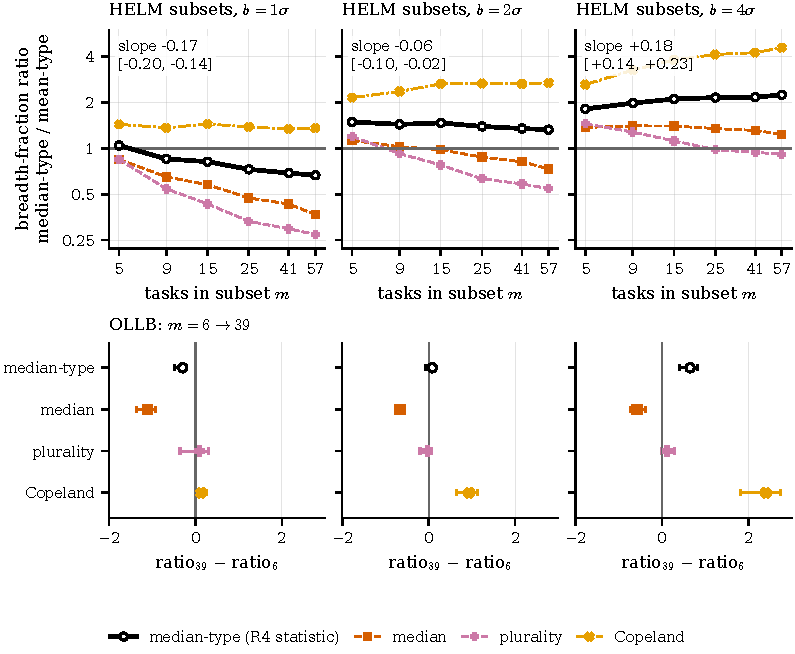
\includegraphics{../figures/fig3_m_effect.pdf}
\caption{Breadth-fraction ratio of the median-type rules to the mean family against the number of tasks $m$ (R4 predicts a rise). Top: random HELM subject subsets (same 79 models) at budgets of one, two (primary) and four task standard deviations; black: the R4 statistic with its slope against $\ln m$. Bottom: Open LLM Leaderboard, change in the ratio from bundled benchmark plans ($m=6$) to free sub-task plans ($m=39$), by rule. Infeasible cells count as breadth fraction 1.}
\label{fig:m}
\end{figure}

\subsection{What predicts the price}
\label{sec:predictors}

The pre-registered prediction R3 is that a rule's gap to the incumbent does not by itself carry the price from one board to another; it is borne out for all seven rules, since each fails in its worst direction (\Cref{tab:verdicts}). The pre-registered test is in raw units: the held-out $R^2$ of log price on the rule's own gap, fitted on one board and tested on another, is negative in the worst of the six directions for six of seven rules (the minimum's is 0.15), and in the best direction reaches 0.85 for the mean, 0.89 for the median and 0.93 for the minimum, and at most 0.24 for the others, so the gap carries the price of the minimum and the median in single directions only. Within a board, with families of models held out in turn, the gap predicts the price at ceilings with a cross-validated $R^2$ of 0.5 to 1.0 for every rule except plurality (0.0 to 0.65): the gap-to-price map is rule- and board-specific, not absent. The mean's failure is by construction (its depth is $m$ times the gap): per task its gap-only $R^2$ is 1.00, while the six other rules still do not transfer (worst direction $-2.9$ to $-1608$; \Cref{app:r3norm}).

We also tested, after R1 and R4 failed, whether summaries of the target's deficit profile (its Gini coefficient, the Lorenz share of its smaller half, the share of tasks within one standard deviation of the incumbent) add to the gap. Retention required a held-out gain of at least 0.1 in $R^2$ with an interval above zero. For the mean the gain is zero (the price is a function of the gap) and the z-mean never retains it. Within a board it holds for the minimum on HELM and at benchmark level and for plurality at benchmark level; across boards it holds in 11 of 122 cases with the intercept re-estimated (37 with the fitted intercept kept, where the gap-only baseline is far below zero). We take the hypothesis as not supported in general.

\subsection{Units, noise and the scale of a boost}
\label{sec:robustness}

\paragraph{Units.}
That the median-type rules are cheaper than the mean family under a cap does not survive a change of unit (R5; \Cref{tab:verdicts}): on HELM they are cheaper in points, in standard deviations and under a convex cost but not as a fraction of headroom; uncapped, they are cheaper in all four units on all boards.

\paragraph{Noise.}
Requiring the aggregate to lead by $c$ noise standard deviations, every top-30 target reaches a 90\% chance of first place under the mean family, the median and the minimum, on HELM and on the sub-task board. The depth at $c=0$ is multiplied by 1.2 to 2.0 for the mean family, 3.4 to 6.2 for the minimum and 6.2 to 6.7 for the median, and the median needs the widest margin ($c=8$ against 3 on HELM, 4 against 2 on the sub-task board; \Cref{app:e6e7}). The other rules were not run with noise.

\paragraph{Calibration of the boost scale.}\label{sec:calibration}
Open LLM Leaderboard fine-tunes with a base model on the board (498 pairs from 76 bases) show median best-task gains of 8 to 9 points for parents under 9B and 27 to 36 points for parents of 9B and above (\Cref{fig:calib}); the budgets that matter (median $B^\ast$ of 2 to 12 points, \Cref{tab:price}) lie within these gains only for parents of 9B and above. For the top targets (mostly 70B and above) and for HELM, which has no pairs, the scale is an assumption.

\begin{table}[t]
\centering
\caption{Pre-registered tests and verdicts, each against the direction predicted (S, P, F: supported, partial, failed). HELM-57 has $m=57$ subjects; OLLB-6 and OLLB-39 are the Open LLM Leaderboard at benchmark ($m=6$) and sub-task ($m=39$) level. The last three rows are exploratory and post hoc.}
\label{tab:verdicts}
\footnotesize\setlength{\tabcolsep}{2.5pt}
\begin{tabular}{@{}>{\raggedright\arraybackslash}p{0.58in}>{\raggedright\arraybackslash}p{0.82in}>{\raggedright\arraybackslash}p{3.2in}>{\raggedright\arraybackslash}p{0.7in}@{}}
\toprule
Scope & Value & 95\% CI / detail & Verdict\\
\midrule
\multicolumn{4}{@{}>{\raggedright\arraybackslash}p{5.4in}}{\emph{R1: median-type rules (median, plurality, Copeland) need more breadth than the mean. Share of targets ($\ge0.8$ predicted); paired difference in $k/m$ [95\% CI] ($>0$ predicted); S/P/F = supported/partial/failed}}\\
HELM-57 & 0.04/0.04/0.28 & $-$0.43\,[$-$0.57,$-$0.29]\hspace{2pt}$-$0.69\,[$-$0.77,$-$0.57]\hspace{2pt}$-$0.08\,[$-$0.12,$-$0.01] & F, F, F\\
OLLB-6 & 0.69/0.66/0.38 & 0.26\,[0.17,0.37]\hspace{2pt}0.22\,[0.16,0.38]\hspace{2pt}0.03\,[$-$0.10,0.14] & P, P, F\\
OLLB-39 & 0.48/1.00/1.00 & 0.08\,[$-$0.01,0.25]\hspace{2pt}0.72\,[0.66,0.86]\hspace{2pt}0.49\,[0.42,0.63] & F, S, S\\
\addlinespace[2pt]\multicolumn{4}{@{}>{\raggedright\arraybackslash}p{5.4in}}{\emph{R2: no rule is cheapest in depth for $\ge90\%$ of targets (largest share over budgets, incumbents)}}\\
each board & \multicolumn{2}{>{\raggedright\arraybackslash}p{4.09in}}{HELM-57 plurality 0.73; OLLB-6 median 0.53; OLLB-39 Borda 0.67} & supported\\
\addlinespace[2pt]\multicolumn{4}{@{}>{\raggedright\arraybackslash}p{5.4in}}{\emph{R3: the gap alone does not predict price (held-out $R^2<0.9$ in the worst of the six directions)}}\\
across & \multicolumn{2}{>{\raggedright\arraybackslash}p{4.09in}}{worst direction per rule: best 0.15, lowest $-1.3\times10^{3}$; $<0$ for 6 of 7} & supported\\
within & \multicolumn{2}{>{\raggedright\arraybackslash}p{4.09in}}{grouped-CV $R^2$ over target families: 0.50--1.00; plurality 0.00--0.65} & --\\
\addlinespace[2pt]\multicolumn{4}{@{}>{\raggedright\arraybackslash}p{5.4in}}{\emph{R4: median/mean breadth ratio rises with $m$ (slope $>0$ predicted; $b=2\sigma$, other $b$ in Fig.~\ref{fig:m})}}\\
HELM & slope vs $\ln m$ & $-$0.058 [$-$0.101, $-$0.018] & failed\\
OLLB & ratio$_{39}-$ratio$_{6}$ & 0.080 [$-$0.063, 0.152] & failed\\
\addlinespace[2pt]\multicolumn{4}{@{}>{\raggedright\arraybackslash}p{5.4in}}{\emph{R5: median-type cheaper in all 4 units and $\tau\ge0.5$: min Kendall $\tau$; units cheaper; cap/no cap; S/P/F}}\\
HELM-57 & 0.73/0.52 & median-type cheaper in 3/4 of 4 units & F/S\\
OLLB-6 & 0.40/0.33 & median-type cheaper in 0/4 of 4 units & P/P\\
OLLB-39 & 0.18/0.50 & median-type cheaper in 2/4 of 4 units & F/P\\
\addlinespace[2pt]\multicolumn{4}{@{}>{\raggedright\arraybackslash}p{5.4in}}{\emph{Crossing budget $B_\times$ ($\sigma$/task) above which the median needs more breadth than the mean (feasible; 95\% CI)}}\\
crossing & \multicolumn{2}{>{\raggedright\arraybackslash}p{4.09in}}{median: HELM-57 2.8 [2.5, 3.4]; OLLB-6 none; OLLB-39 0.8 [0.7, 0.9]; plurality: HELM-57 none} & --\\
\addlinespace[2pt]\multicolumn{4}{@{}>{\raggedright\arraybackslash}p{5.4in}}{\emph{Deficit-profile test (exploratory, post hoc): profile adds $\ge0.1$ held-out $R^2$ to the gap (CI above 0); cross-board, intercept re-estimated}}\\
profile & \multicolumn{2}{>{\raggedright\arraybackslash}p{4.09in}}{retained in 11 of 122 cases (37 with the fitted intercept kept): median 2, min 4, plurality 5; mean: gain 0 (identity); z-mean: never retained} & not supported\\
\bottomrule
\end{tabular}
% source: \texttt{results/verdicts.csv}, \texttt{results/predictors_within.csv}, \texttt{results/bx_crossing.csv}, \texttt{results/predictors_hl.csv}

\end{table}

\section{Discussion and limitations}
\label{sec:discussion}

\paragraph{What the results say about rule choice.}
First place has two prices, and which rule makes it dearer depends on which binds. If total effort is the constraint, the mean family is the dearest rule on every board (\Cref{sec:pricemap}), because its depth is $m$ times the gap. If effort per task is the constraint, the hardest rule to buy is the minimum on HELM (median minimal feasible budget 11 points, against 6.5 for the mean and 2.7 for plurality) and plurality on the Open LLM Leaderboard (9 and 12 points), and the order moves with the budget (\Cref{sec:breadth}). To make first place costly in total points, average; to demand capability on every task, take the minimum.

\paragraph{Scope.}
The conclusions hold for three boards, 30 top targets, the boost model of \Cref{sec:setting} and budgets seen for fine-tunes of models of 9B and above. Comparisons by total boost are robust to the incumbent on HELM and to the unit when uncapped; those by breadth are not.
\emph{The developer} is a single, static actor: rivals do not respond, so the prices are a lower envelope of the cost on a contested board. \emph{The boost} is an input whose scale is checked, not produced, by training; boosts on different tasks are independent, and a spillover-aware variant lowers the cheapest total boost to 92--95\% of the independent one. \emph{Boards}: HELM is one benchmark family and the Open LLM Leaderboard's top a crowd of derivatives, so each comparison has 11--13 independent clusters.

\paragraph{Impact.}
The prices show how cheaply a board can be gamed; we train nothing and release only an analysis of public scores.


\bibliographystyle{plainnat}
\bibliography{refs}

\appendix

\section{Proofs}
\label{app:proofs}

Throughout, $t$ is the target, $\delta_j\in[0,u_j]$ with $u_j=\min(B,c_j-S_{tj})$ is the boost on task $j$, and a rival $i$ is beaten when the target's aggregate exceeds theirs by $\varepsilon$.

\paragraph{\Cref{prop:quantile}.}
Let the rival level be $V$, the largest rival aggregate plus $\varepsilon$. The $r$-th largest of the target's scores is at least $V$ if and only if at least $r$ of them are. The $a$ tasks already at $V$ or above count, so at least $r-a$ further tasks must be raised to $V$, which is the stated breadth. Raising a task from $S_{tj}$ to $V$ costs $d_j=V-S_{tj}$, and raising it beyond $V$, or raising a task that ends below $V$, does not help any of the $r$ positions that matter. For a set $T$ of $r-a$ tasks the least depth is $\sum_{j\in T}d_j$, minimised by the $r-a$ smallest shortfalls (exchange argument: swapping a chosen task for an unchosen one with smaller shortfall lowers the sum). The plan is feasible under $B$ and the ceilings if and only if each chosen $d_j\le u_j$, and the best choice is feasible if and only if the $(r-a)$-th smallest value of the shortfalls among tasks with $d_j\le u_j$ exists, which for tasks with equal ceilings is the condition on the $(r-a)$-th smallest shortfall stated in the proposition. The minimum is $r=m$ and the median is $r=\lceil m/2\rceil$.

\paragraph{\Cref{prop:mean}.}
With weights $w_j>0$ the target's aggregate is $A_t+\sum_jw_j\delta_j$ and first place requires $\sum_jw_j\delta_j\ge G$ (strictly, with the margin $\varepsilon$ included in $G$). The set of feasible $\delta$ is the knapsack cover $\{0\le\delta_j\le u_j,\sum_jw_j\delta_j\ge G\}$ and is non-empty if and only if $\sum_jw_ju_j\ge G$. With a linear cost $\sum_j\kappa_j\delta_j$ it is a fractional covering problem, solved by filling tasks in decreasing order of $w_j/\kappa_j$ until $G$ is covered. For the raw mean in points $w_j=1/m$ and $\kappa_j=1$, so every unit of boost buys the same $1/m$ of aggregate and the depth is $mG$ however the boost is spread. The least number of tasks that covers $G$ is the least $k$ with $\sum$ of the $k$ largest $w_ju_j$ at least $G$, because with unit cost per task it is best to take the largest headrooms. Under a convex cost the optimum equalises marginal cost per unit of aggregate across tasks that are not at their cap (water-filling).

\paragraph{\Cref{prop:rank}.}
Let the target's win count against rival $i$ on task $j$ be $1[S_{tj}>S_{ij}]+\tfrac12 1[S_{tj}=S_{ij}]$; mean rank is the sum over rivals and tasks of this quantity, divided by $m(N-1)$, and ties counted as half give the mean win rate. As a function of $\delta_j$ the count against $i$ is a non-decreasing step function that changes at $S_{ij}-S_{tj}$, so the target's total on task $j$ is a step function with one step for each rival whose score is passed, at most $N-1$ steps, and no step beyond the best rival's score on $j$. The condition to be ahead of rival $i$ is that the sum over tasks of the margin steps against $i$ is at least the deficit $g_i$, and ahead of every rival means all such constraints hold together. Choosing for each task one level from the finite set of steps is a multiple-choice covering problem with one constraint for each rival, with cost $\sum_j\delta_j$. Each task adds at most $N$ pairwise wins against any given rival, so at least $\lceil g_i/N\rceil$ tasks must be raised.

\paragraph{\Cref{prop:coupled}.}
Plurality: the target wins task $j$ if it has the highest score there, so it must pass the best rival on that task, and the winner count of that rival falls by one. The target leads rival $i$ if its number of task wins exceeds the rival's, and the rival's wins also depend on which tasks the target takes. Copeland: the target beats rival $i$ if it passes them on more tasks than they pass it; its score is the number of rivals beaten (ties count half), and first place requires it to exceed every rival's score, which themselves change with the target's boost. In both rules the effect of boosting task $j$ depends on which other tasks are boosted, so the problem does not decompose by task and is stated as a mixed-integer program with one constraint for each rival and a binary choice of level for each task.

\paragraph{No-dominance instances.}
Target $(59,59,0)$ against rival $(60,60,60)$: the median is $59$ against $60$, and raising two tasks to $60+\varepsilon$ gives a median of $60+\varepsilon$ for a depth of about $2$; the means are $39.3$ and $60$, a gap of $20.7$ and a depth of $62$ (\Cref{prop:mean}). Target $(100,0,0)$ against rival $(0,50,50)$: the means are $33.3$ and $33.3$, so a boost of order $\varepsilon$ makes the target first under the mean, whereas the median is $0$ against $50$ and the target needs a task raised from $0$ to $50+\varepsilon$, a depth of about $50$.

\section{Naive developers}
\label{app:e5}

The optimum of the main text is the cost of a perfectly targeted developer. \Cref{tab:e5} compares it with four rules of thumb at $B=10$ points on the 30 highest-ranked targets: \emph{greedy} (repeatedly raise the task that moves the target's rule score most), \emph{hardest} (raise tasks in ascending order of the target's own score), \emph{random} (random order of tasks) and \emph{uniform} (the same boost on every task). Each developer stops at the first plan that makes the target first. The table gives the median over targets of the ratio of the developer's depth to the optimum. The mean gives a ratio of 1 by construction, and the rules that reward targeting (median, minimum, plurality, Copeland) cost an untargeted developer between 1.2 and 53 times the optimum, in most cells more than 3 times.

\begin{table}[h]
\caption{Median ratio of a developer's depth to the optimal depth, $B=10$ points, top-30 targets.}
\label{tab:e5}
\centering\footnotesize
\begin{tabular}{llrrrr}
\toprule
Board & Rule & Greedy & Hardest & Random & Uniform\\
\midrule
HELM & mean & 1.0 & 1.0 & 1.0 & 1.0\\
HELM & $z$-mean & 1.1 & 1.8 & 1.5 & 1.5\\
HELM & Borda & 2.0 & 2.6 & 2.5 & 1.6\\
HELM & Copeland & 4.0 & 4.0 & 3.4 & 2.9\\
HELM & median & 6.8 & 9.3 & 9.4 & 8.8\\
HELM & minimum & 2.2 & 2.2 & 53 & 34\\
HELM & plurality & 4.9 & 14.6 & 6.7 & 9.5\\
\midrule
Sub-task & mean & 1.0 & 1.0 & 1.0 & 1.0\\
Sub-task & $z$-mean & 1.0 & 1.7 & 1.9 & 1.8\\
Sub-task & Borda & 2.2 & 3.7 & 3.8 & 2.2\\
Sub-task & Copeland & 6.3 & 7.3 & 6.8 & 6.4\\
Sub-task & median & 5.5 & 29.5 & 20.0 & 18.5\\
Sub-task & minimum & 1.2 & 1.2 & 20.7 & 25.2\\
Sub-task & plurality & 3.9 & 8.1 & 8.3 & 11.2\\
\bottomrule
\end{tabular}
\end{table}

\section{Noise, margins and spillover}
\label{app:e6e7}

\paragraph{Noise.}
Noise runs use the 60 highest-ranked models of each noisy board and the 30 highest-ranked as targets. Every (model, task) score of every model, rivals included, receives independent Gaussian noise clipped to $[0,100]$: on HELM the binomial standard deviation $100\sqrt{p(1-p)/n}$ with $n$ the number of items of the subject, on the sub-task board the reported standard error. For the mean, z-mean, median and minimum, ``leading by $c$ standard deviations'' means that the noise-free aggregate of the cheapest plan beats the best other model's by $c\,s$, where $s$ is the standard deviation, over 400 noisy draws, of the difference of the rule's own aggregate between the target and that model; it is measured on the unboosted board, and re-solving with the standard deviation of the boosted plan gives the same picture (second entry of each pair in \Cref{tab:noise}). The probability of first place is the share of 400 draws in which the boosted target beats all 59 others (Monte-Carlo standard error at most 0.025). The margin grid runs to $c=12$. Plurality, Borda and Copeland have no such margin and were run at $c=0$ only.

\begin{table}[h]
\centering
\caption{Confidence of 90\% for first place under noise (top 30 targets): median over targets of the smallest margin $c$ at which a target reaches it (all 30 reach it within the grid), and the depth at that $c$ relative to the depth at $c=0$ (median over targets). Margin from the unboosted / the boosted plan's standard deviation.}
\label{tab:noise}
\small
\begin{tabular}{lcccc}
\toprule
 & \multicolumn{2}{c}{HELM} & \multicolumn{2}{c}{sub-task board} \\
rule & $c$ & depth ratio & $c$ & depth ratio \\
\midrule
mean & 3 / 3 & 1.26 / 1.21 & 2 / 2 & 1.66 / 1.62 \\
z-mean & 3 / 3 & 1.44 / 1.39 & 2 / 2 & 1.98 / 2.04 \\
median & 8 / 5 & 6.7 / 6.2 & 4 / 4 & 6.7 / 6.4 \\
min & 3 / 4 & 5.3 / 6.2 & 3 / 3 & 3.7 / 3.4 \\
\bottomrule
\end{tabular}
\end{table}

\paragraph{Margin and rivals.}
All sensitivity runs are on the benchmark-level board. The main analysis uses $\varepsilon=10^{-6}$ points. With $\varepsilon=0.1$ the median depth at $B=10$ rises by 2 to 4\% for every rule, and with $\varepsilon=1$ by 2 to 42\% (most for the median and Copeland); the order of the rules by median depth keeps a Kendall $\tau$ of 1.00 with $\varepsilon=0.1$ and 0.71 with $\varepsilon=1$. Keeping merged, flagged and off-hub models as rivals (4576 models) leaves the order at $\tau=0.90$.

\paragraph{Spillover.}
A boost on one benchmark also moves others. Using the measured gains of base--fine-tune pairs on the other benchmarks as spillover coefficients, the cheapest total boost under the mean falls to 0.95, 0.94 and 0.92 of the independent price at $B=5$, 10 and 100 points (median over targets), a small change.

\paragraph{Transfer across boards on normalised quantities.}\label{app:r3norm}
\Cref{tab:r3norm} repeats the transfer test of R3 (post hoc variants; the raw-unit test is the pre-registered one) on price per task, $\log(\text{depth}/m)$ on $\log$ gap, in the worst and the best of the six fit--test directions, and, in the last column, the lowest of the six directions with the intercept re-estimated on the test board.

\begin{table}[h]
\centering
\caption{Held-out $R^2$ of log price on log gap across boards: raw units (pre-registered) and per task; worst / best of six directions; last column the lowest of the six directions with the intercept re-estimated on the test board (identical for raw and per task, since the intercept absorbs $\log m$).}
\label{tab:r3norm}
\small
\begin{tabular}{lccc}
\toprule
rule & raw & per task & re-estimated \\
\midrule
mean & $-17.7$ / 0.85 & 1.00 / 1.00 & 1.00 \\
z-mean & $-41.4$ / $-0.15$ & $-12.8$ / 0.82 & 0.97 \\
median & $-0.59$ / 0.89 & $-2.9$ / 0.66 & 0.62 \\
min & 0.15 / 0.93 & $-3.6$ / 0.87 & 0.68 \\
Borda & $-24.9$ / 0.23 & $-47$ / 0.75 & $-3.4$ \\
plurality & $-1294$ / 0.24 & $-1608$ / 0.17 & $-3.1$ \\
Copeland & $-5.0$ / 0.06 & $-3.7$ / 0.66 & $-3.7$ \\
\bottomrule
\end{tabular}
\end{table}

\section{Further figures}
\label{app:figs}

\begin{figure}[h]
\centering
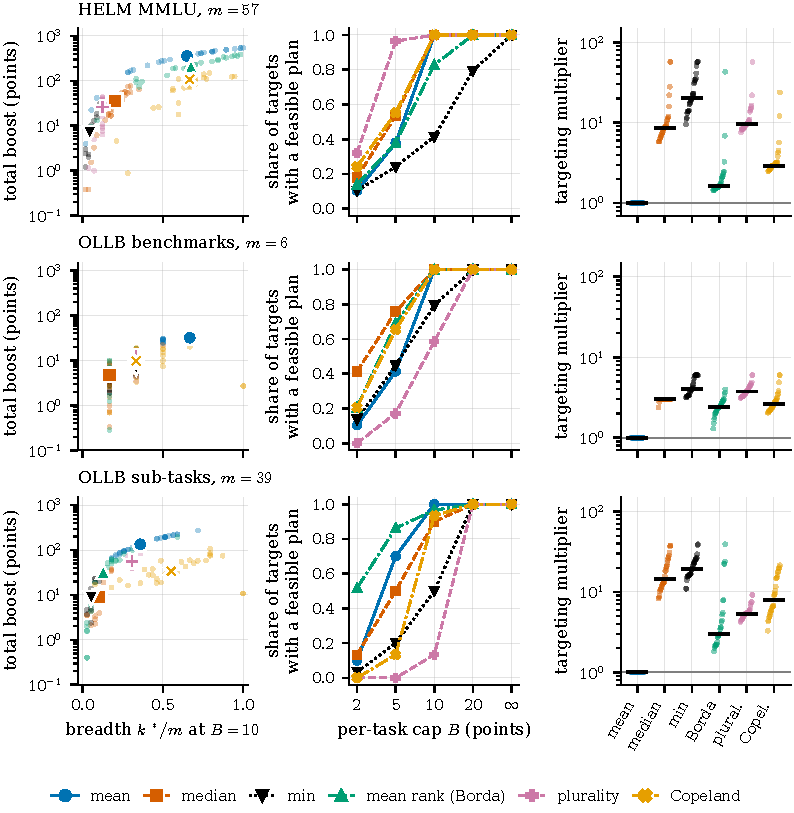
\includegraphics{../figures/fig2_price_map.pdf}
\caption{Price of first place for the 30 highest-ranked targets of each board (rows), against each rule's own leader; targets with zero gap are omitted. Left: total boost against breadth fraction at a per-task cap of 10 points (axes clipped at the bottom; one HELM and two benchmark-level targets within the tie margin of first place are off scale). Centre: share of targets with a feasible plan against the per-task cap. Right: targeting multiplier, the depth of the cheapest uniform plan over that of the cheapest targeted plan, at ceilings (two HELM and two sub-task targets off scale).}
\label{fig:map}
\end{figure}

\begin{figure}[h]
\centering
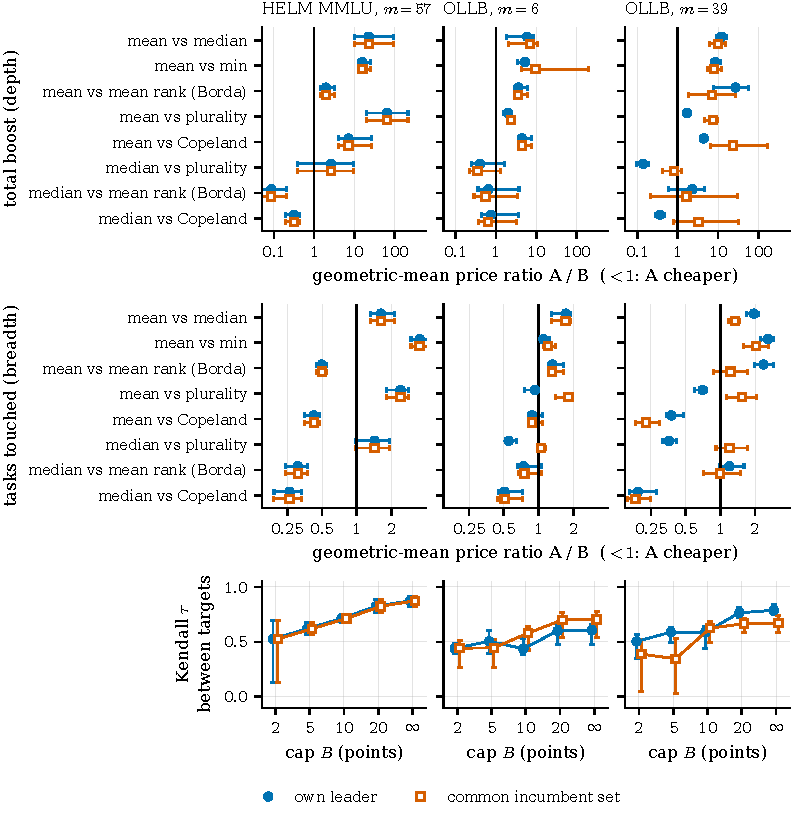
\includegraphics{../figures/fig4_pairs.pdf}
\caption{Paired price ratios between rules at a per-task cap of 20 points: geometric mean over targets of the price of the first rule divided by that of the second, with cluster-bootstrap 95\% intervals, for total boost (top) and for tasks touched (bottom), against each rule's own leader and a common incumbent set. Each cell uses 21--30 targets (targets already first under a rule are dropped). Ratios on the two sides of 1 show that no rule is cheapest throughout. The bottom row of panels shows the mean Kendall $\tau$ between the rule orderings of two targets against the per-task cap, with cluster-bootstrap 95\% intervals, again for own and common incumbents; it rises with the cap.}
\label{fig:paired}
\end{figure}

\begin{figure}[h]
\centering
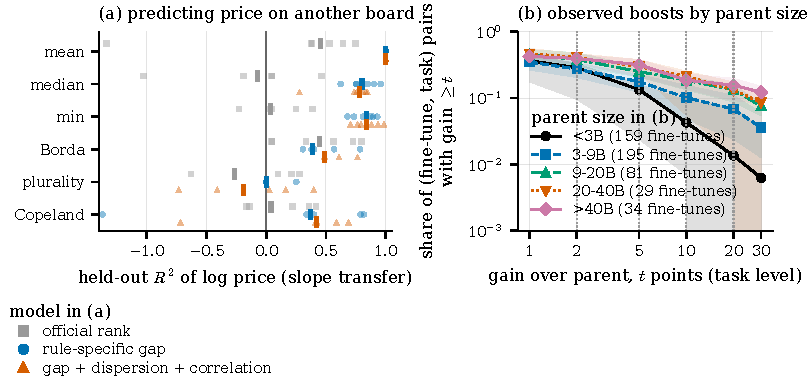
\includegraphics{../figures/fig5_predictors_calibration.pdf}
\caption{(a) Held-out $R^2$ of log price at ceilings when a model fitted on one board is applied to another with the slope transferred and the intercept re-estimated (the raw $R^2$ quoted for R3 is in \Cref{tab:verdicts}); 14 of 126 cells fall below $-1.4$ and are off the left edge. (b) Observed gains of fine-tuned models over their base models on the Open LLM Leaderboard: share of fine-tunes with a gain of at least a given number of points on some task, by parent size; grid lines at the budgets 2, 5, 10 and 20.}
\label{fig:calib}
\end{figure}

Detail of the calibration of \Cref{sec:calibration}. Open LLM Leaderboard models with a base model on the board give 159, 195, 81, 29 and 34 base--fine-tune pairs (from 21, 29, 13, 6 and 7 bases) for parents under 3B, 3--9B, 9--20B, 20--40B and over 40B. The median over children of the largest gain on any benchmark is 8, 9, 27, 34 and 36 points in these buckets, and the share of single-benchmark gains of at least 10 points rises from 4\% to 19--21\%. The budgets that matter (median minimal feasible budgets $B^\ast$ of 2 to 12 points, \Cref{tab:price}) lie within the range of the observed best-task gains only for parents of 9B and above: for 3--9B parents the median best-task gain is 9.3 (interval 5.7 to 20.0), below the larger budgets (11.5 for the minimum on HELM, 9.2 and 11.9 for plurality on the Open LLM Leaderboard). The top-30 targets are mostly models of 70B and above, for which the over-40B bucket has 34 children from 7 bases, and HELM's models have no observed pairs at all, so for them the scale is an assumption (\Cref{sec:discussion}); the pairs are not randomised, and a parent that is on the board is not always the model that was fine-tuned.

\section{Release and reproduction}
\label{app:release}

Every number in the paper is produced from the released analysis code and the result tables, which are anonymised for review. The inputs are the frozen public snapshots listed in \Cref{sec:data}: HELM MMLU release v1.13.0, and the Open LLM Leaderboard \texttt{contents} and \texttt{results} datasets at the commits given there. The code runs on CPU with Python 3.11, numpy 2.4, scipy 1.17, pandas 3.0 and HiGHS 1.16, and the random draws use fixed seeds. The exact price runs are the expensive part, about 77\,000 solver seconds in total on a shared CPU host (a few seconds to a half minute per target and rule on the largest boards, with a 30\,s limit per integer program); the figure is an upper bound on CPU time because the host was loaded. The licences of the data are those of their sources, and only processed numbers are redistributed.


\section*{NeurIPS Paper Checklist}




\begin{enumerate}

\item {\bf Claims}
    \item[] Question: Do the main claims made in the abstract and introduction accurately reflect the paper's contributions and scope?
    \item[] Answer: \answerYes{}
    \item[] Justification: The abstract and introduction state the price of first place, the three public boards and the results, including the pre-registered expectations that fail (\Cref{sec:intro,sec:results}).
    \item[] Guidelines:
    \begin{itemize}
        \item The answer \answerNA{} means that the abstract and introduction do not include the claims made in the paper.
        \item The abstract and/or introduction should clearly state the claims made, including the contributions made in the paper and important assumptions and limitations. A \answerNo{} or \answerNA{} answer to this question will not be perceived well by the reviewers. 
        \item The claims made should match theoretical and experimental results, and reflect how much the results can be expected to generalize to other settings. 
        \item It is fine to include aspirational goals as motivation as long as it is clear that these goals are not attained by the paper. 
    \end{itemize}

\item {\bf Limitations}
    \item[] Question: Does the paper discuss the limitations of the work performed by the authors?
    \item[] Answer: \answerYes{}
    \item[] Justification: \Cref{sec:discussion} states where the conclusions hold and where not: a static single developer, an assumed boost scale outside the observed fine-tunes, three boards, few independent clusters, and solver optimality gaps.
    \item[] Guidelines:
    \begin{itemize}
        \item The answer \answerNA{} means that the paper has no limitation while the answer \answerNo{} means that the paper has limitations, but those are not discussed in the paper. 
        \item The authors are encouraged to create a separate ``Limitations'' section in their paper.
        \item The paper should point out any strong assumptions and how robust the results are to violations of these assumptions (e.g., independence assumptions, noiseless settings, model well-specification, asymptotic approximations only holding locally). The authors should reflect on how these assumptions might be violated in practice and what the implications would be.
        \item The authors should reflect on the scope of the claims made, e.g., if the approach was only tested on a few datasets or with a few runs. In general, empirical results often depend on implicit assumptions, which should be articulated.
        \item The authors should reflect on the factors that influence the performance of the approach. For example, a facial recognition algorithm may perform poorly when image resolution is low or images are taken in low lighting. Or a speech-to-text system might not be used reliably to provide closed captions for online lectures because it fails to handle technical jargon.
        \item The authors should discuss the computational efficiency of the proposed algorithms and how they scale with dataset size.
        \item If applicable, the authors should discuss possible limitations of their approach to address problems of privacy and fairness.
        \item While the authors might fear that complete honesty about limitations might be used by reviewers as grounds for rejection, a worse outcome might be that reviewers discover limitations that aren't acknowledged in the paper. The authors should use their best judgment and recognize that individual actions in favor of transparency play an important role in developing norms that preserve the integrity of the community. Reviewers will be specifically instructed to not penalize honesty concerning limitations.
    \end{itemize}

\item {\bf Theory assumptions and proofs}
    \item[] Question: For each theoretical result, does the paper provide the full set of assumptions and a complete (and correct) proof?
    \item[] Answer: \answerYes{}
    \item[] Justification: Assumptions are in \Cref{sec:setting} and in each statement; proofs are in \Cref{app:proofs}, with sketches in \Cref{sec:exact}.
    \item[] Guidelines:
    \begin{itemize}
        \item The answer \answerNA{} means that the paper does not include theoretical results. 
        \item All the theorems, formulas, and proofs in the paper should be numbered and cross-referenced.
        \item All assumptions should be clearly stated or referenced in the statement of any theorems.
        \item The proofs can either appear in the main paper or the supplemental material, but if they appear in the supplemental material, the authors are encouraged to provide a short proof sketch to provide intuition. 
        \item Inversely, any informal proof provided in the core of the paper should be complemented by formal proofs provided in appendix or supplemental material.
        \item Theorems and Lemmas that the proof relies upon should be properly referenced. 
    \end{itemize}

    \item {\bf Experimental result reproducibility}
    \item[] Question: Does the paper fully disclose all the information needed to reproduce the main experimental results of the paper to the extent that it affects the main claims and/or conclusions of the paper (regardless of whether the code and data are provided or not)?
    \item[] Answer: \answerYes{}
    \item[] Justification: \Cref{sec:setting,sec:data} define the price, the boards, the targets, the budgets and the tests; \Cref{app:release} gives the environment and seeds.
    \item[] Guidelines:
    \begin{itemize}
        \item The answer \answerNA{} means that the paper does not include experiments.
        \item If the paper includes experiments, a \answerNo{} answer to this question will not be perceived well by the reviewers: Making the paper reproducible is important, regardless of whether the code and data are provided or not.
        \item If the contribution is a dataset and\slash or model, the authors should describe the steps taken to make their results reproducible or verifiable. 
        \item Depending on the contribution, reproducibility can be accomplished in various ways. For example, if the contribution is a novel architecture, describing the architecture fully might suffice, or if the contribution is a specific model and empirical evaluation, it may be necessary to either make it possible for others to replicate the model with the same dataset, or provide access to the model. In general. releasing code and data is often one good way to accomplish this, but reproducibility can also be provided via detailed instructions for how to replicate the results, access to a hosted model (e.g., in the case of a large language model), releasing of a model checkpoint, or other means that are appropriate to the research performed.
        \item While NeurIPS does not require releasing code, the conference does require all submissions to provide some reasonable avenue for reproducibility, which may depend on the nature of the contribution. For example
        \begin{enumerate}
            \item If the contribution is primarily a new algorithm, the paper should make it clear how to reproduce that algorithm.
            \item If the contribution is primarily a new model architecture, the paper should describe the architecture clearly and fully.
            \item If the contribution is a new model (e.g., a large language model), then there should either be a way to access this model for reproducing the results or a way to reproduce the model (e.g., with an open-source dataset or instructions for how to construct the dataset).
            \item We recognize that reproducibility may be tricky in some cases, in which case authors are welcome to describe the particular way they provide for reproducibility. In the case of closed-source models, it may be that access to the model is limited in some way (e.g., to registered users), but it should be possible for other researchers to have some path to reproducing or verifying the results.
        \end{enumerate}
    \end{itemize}


\item {\bf Open access to data and code}
    \item[] Question: Does the paper provide open access to the data and code, with sufficient instructions to faithfully reproduce the main experimental results, as described in supplemental material?
    \item[] Answer: \answerYes{}
    \item[] Justification: The anonymised code, the result tables and the commands that rebuild every number are released; the inputs are frozen public snapshots (\Cref{app:release}).
    \item[] Guidelines:
    \begin{itemize}
        \item The answer \answerNA{} means that paper does not include experiments requiring code.
        \item Please see the NeurIPS code and data submission guidelines (\url{https://neurips.cc/public/guides/CodeSubmissionPolicy}) for more details.
        \item While we encourage the release of code and data, we understand that this might not be possible, so \answerNo{} is an acceptable answer. Papers cannot be rejected simply for not including code, unless this is central to the contribution (e.g., for a new open-source benchmark).
        \item The instructions should contain the exact command and environment needed to run to reproduce the results. See the NeurIPS code and data submission guidelines (\url{https://neurips.cc/public/guides/CodeSubmissionPolicy}) for more details.
        \item The authors should provide instructions on data access and preparation, including how to access the raw data, preprocessed data, intermediate data, and generated data, etc.
        \item The authors should provide scripts to reproduce all experimental results for the new proposed method and baselines. If only a subset of experiments are reproducible, they should state which ones are omitted from the script and why.
        \item At submission time, to preserve anonymity, the authors should release anonymized versions (if applicable).
        \item Providing as much information as possible in supplemental material (appended to the paper) is recommended, but including URLs to data and code is permitted.
    \end{itemize}


\item {\bf Experimental setting/details}
    \item[] Question: Does the paper specify all the training and test details (e.g., data splits, hyperparameters, how they were chosen, type of optimizer) necessary to understand the results?
    \item[] Answer: \answerYes{}
    \item[] Justification: No model is trained. The boards, the targets, the budget grid, the margin, the incumbents and the bootstrap are specified in \Cref{sec:data}, and the sensitivity to the margin is in \Cref{app:e6e7}.
    \item[] Guidelines:
    \begin{itemize}
        \item The answer \answerNA{} means that the paper does not include experiments.
        \item The experimental setting should be presented in the core of the paper to a level of detail that is necessary to appreciate the results and make sense of them.
        \item The full details can be provided either with the code, in appendix, or as supplemental material.
    \end{itemize}

\item {\bf Experiment statistical significance}
    \item[] Question: Does the paper report error bars suitably and correctly defined or other appropriate information about the statistical significance of the experiments?
    \item[] Answer: \answerYes{}
    \item[] Justification: Comparisons across targets carry cluster bootstrap intervals by incumbent and family, and the number of independent clusters is stated (\Cref{sec:data,sec:results}); price tables are medians over targets without interval.
    \item[] Guidelines:
    \begin{itemize}
        \item The answer \answerNA{} means that the paper does not include experiments.
        \item The authors should answer \answerYes{} if the results are accompanied by error bars, confidence intervals, or statistical significance tests, at least for the experiments that support the main claims of the paper.
        \item The factors of variability that the error bars are capturing should be clearly stated (for example, train/test split, initialization, random drawing of some parameter, or overall run with given experimental conditions).
        \item The method for calculating the error bars should be explained (closed form formula, call to a library function, bootstrap, etc.)
        \item The assumptions made should be given (e.g., Normally distributed errors).
        \item It should be clear whether the error bar is the standard deviation or the standard error of the mean.
        \item It is OK to report 1-sigma error bars, but one should state it. The authors should preferably report a 2-sigma error bar than state that they have a 96\% CI, if the hypothesis of Normality of errors is not verified.
        \item For asymmetric distributions, the authors should be careful not to show in tables or figures symmetric error bars that would yield results that are out of range (e.g., negative error rates).
        \item If error bars are reported in tables or plots, the authors should explain in the text how they were calculated and reference the corresponding figures or tables in the text.
    \end{itemize}

\item {\bf Experiments compute resources}
    \item[] Question: For each experiment, does the paper provide sufficient information on the computer resources (type of compute workers, memory, time of execution) needed to reproduce the experiments?
    \item[] Answer: \answerYes{}
    \item[] Justification: CPU only; \Cref{app:release} gives the environment and about 77\,000 solver seconds in total on a shared host, which is more than the 4 CPU-hours we planned, mostly in the exact programs for HELM and the 39-task board.
    \item[] Guidelines:
    \begin{itemize}
        \item The answer \answerNA{} means that the paper does not include experiments.
        \item The paper should indicate the type of compute workers CPU or GPU, internal cluster, or cloud provider, including relevant memory and storage.
        \item The paper should provide the amount of compute required for each of the individual experimental runs as well as estimate the total compute. 
        \item The paper should disclose whether the full research project required more compute than the experiments reported in the paper (e.g., preliminary or failed experiments that didn't make it into the paper). 
    \end{itemize}
    
\item {\bf Code of ethics}
    \item[] Question: Does the research conducted in the paper conform, in every respect, with the NeurIPS Code of Ethics \url{https://neurips.cc/public/EthicsGuidelines}?
    \item[] Answer: \answerYes{}
    \item[] Justification: The work uses public score tables only, with no human subjects and no training, and follows the NeurIPS Code of Ethics.
    \item[] Guidelines:
    \begin{itemize}
        \item The answer \answerNA{} means that the authors have not reviewed the NeurIPS Code of Ethics.
        \item If the authors answer \answerNo, they should explain the special circumstances that require a deviation from the Code of Ethics.
        \item The authors should make sure to preserve anonymity (e.g., if there is a special consideration due to laws or regulations in their jurisdiction).
    \end{itemize}


\item {\bf Broader impacts}
    \item[] Question: Does the paper discuss both potential positive societal impacts and negative societal impacts of the work performed?
    \item[] Answer: \answerYes{}
    \item[] Justification: \Cref{sec:discussion} discusses the use of the measurement to help board designers weigh aggregation rules, and that it can also be read as a statement of how cheaply a board can be gamed.
    \item[] Guidelines:
    \begin{itemize}
        \item The answer \answerNA{} means that there is no societal impact of the work performed.
        \item If the authors answer \answerNA{} or \answerNo, they should explain why their work has no societal impact or why the paper does not address societal impact.
        \item Examples of negative societal impacts include potential malicious or unintended uses (e.g., disinformation, generating fake profiles, surveillance), fairness considerations (e.g., deployment of technologies that could make decisions that unfairly impact specific groups), privacy considerations, and security considerations.
        \item The conference expects that many papers will be foundational research and not tied to particular applications, let alone deployments. However, if there is a direct path to any negative applications, the authors should point it out. For example, it is legitimate to point out that an improvement in the quality of generative models could be used to generate Deepfakes for disinformation. On the other hand, it is not needed to point out that a generic algorithm for optimizing neural networks could enable people to train models that generate Deepfakes faster.
        \item The authors should consider possible harms that could arise when the technology is being used as intended and functioning correctly, harms that could arise when the technology is being used as intended but gives incorrect results, and harms following from (intentional or unintentional) misuse of the technology.
        \item If there are negative societal impacts, the authors could also discuss possible mitigation strategies (e.g., gated release of models, providing defenses in addition to attacks, mechanisms for monitoring misuse, mechanisms to monitor how a system learns from feedback over time, improving the efficiency and accessibility of ML).
    \end{itemize}
    
\item {\bf Safeguards}
    \item[] Question: Does the paper describe safeguards that have been put in place for responsible release of data or models that have a high risk for misuse (e.g., pre-trained language models, image generators, or scraped datasets)?
    \item[] Answer: \answerNA{}
    \item[] Justification: No model or dataset with a risk of misuse is released; only analysis of public scores.
    \item[] Guidelines:
    \begin{itemize}
        \item The answer \answerNA{} means that the paper poses no such risks.
        \item Released models that have a high risk for misuse or dual-use should be released with necessary safeguards to allow for controlled use of the model, for example by requiring that users adhere to usage guidelines or restrictions to access the model or implementing safety filters. 
        \item Datasets that have been scraped from the Internet could pose safety risks. The authors should describe how they avoided releasing unsafe images.
        \item We recognize that providing effective safeguards is challenging, and many papers do not require this, but we encourage authors to take this into account and make a best faith effort.
    \end{itemize}

\item {\bf Licenses for existing assets}
    \item[] Question: Are the creators or original owners of assets (e.g., code, data, models), used in the paper, properly credited and are the license and terms of use explicitly mentioned and properly respected?
    \item[] Answer: \answerYes{}
    \item[] Justification: HELM, the Open LLM Leaderboard, its six benchmarks and the evaluation harness are cited, and the snapshots are cited by version (\Cref{sec:data}). The HELM code is Apache-2.0 and we found no separate licence for its results; the two Open LLM Leaderboard datasets declare none (the \texttt{contents} table lists each model's Hub licence, and the \texttt{results} repository has no dataset card), so we use them for analysis only and redistribute processed numbers, not the raw tables.
    \item[] Guidelines:
    \begin{itemize}
        \item The answer \answerNA{} means that the paper does not use existing assets.
        \item The authors should cite the original paper that produced the code package or dataset.
        \item The authors should state which version of the asset is used and, if possible, include a URL.
        \item The name of the license (e.g., CC-BY 4.0) should be included for each asset.
        \item For scraped data from a particular source (e.g., website), the copyright and terms of service of that source should be provided.
        \item If assets are released, the license, copyright information, and terms of use in the package should be provided. For popular datasets, \url{paperswithcode.com/datasets} has curated licenses for some datasets. Their licensing guide can help determine the license of a dataset.
        \item For existing datasets that are re-packaged, both the original license and the license of the derived asset (if it has changed) should be provided.
        \item If this information is not available online, the authors are encouraged to reach out to the asset's creators.
    \end{itemize}

\item {\bf New assets}
    \item[] Question: Are new assets introduced in the paper well documented and is the documentation provided alongside the assets?
    \item[] Answer: \answerYes{}
    \item[] Justification: The released result tables and code are documented in the code README; they contain only processed public scores and no author information.
    \item[] Guidelines:
    \begin{itemize}
        \item The answer \answerNA{} means that the paper does not release new assets.
        \item Researchers should communicate the details of the dataset\slash code\slash model as part of their submissions via structured templates. This includes details about training, license, limitations, etc. 
        \item The paper should discuss whether and how consent was obtained from people whose asset is used.
        \item At submission time, remember to anonymize your assets (if applicable). You can either create an anonymized URL or include an anonymized zip file.
    \end{itemize}

\item {\bf Crowdsourcing and research with human subjects}
    \item[] Question: For crowdsourcing experiments and research with human subjects, does the paper include the full text of instructions given to participants and screenshots, if applicable, as well as details about compensation (if any)? 
    \item[] Answer: \answerNA{}
    \item[] Justification: The paper involves no crowdsourcing or research with human subjects.
    \item[] Guidelines:
    \begin{itemize}
        \item The answer \answerNA{} means that the paper does not involve crowdsourcing nor research with human subjects.
        \item Including this information in the supplemental material is fine, but if the main contribution of the paper involves human subjects, then as much detail as possible should be included in the main paper. 
        \item According to the NeurIPS Code of Ethics, workers involved in data collection, curation, or other labor should be paid at least the minimum wage in the country of the data collector. 
    \end{itemize}

\item {\bf Institutional review board (IRB) approvals or equivalent for research with human subjects}
    \item[] Question: Does the paper describe potential risks incurred by study participants, whether such risks were disclosed to the subjects, and whether Institutional Review Board (IRB) approvals (or an equivalent approval/review based on the requirements of your country or institution) were obtained?
    \item[] Answer: \answerNA{}
    \item[] Justification: The paper involves no crowdsourcing or research with human subjects, so no review board approval applies.
    \item[] Guidelines:
    \begin{itemize}
        \item The answer \answerNA{} means that the paper does not involve crowdsourcing nor research with human subjects.
        \item Depending on the country in which research is conducted, IRB approval (or equivalent) may be required for any human subjects research. If you obtained IRB approval, you should clearly state this in the paper. 
        \item We recognize that the procedures for this may vary significantly between institutions and locations, and we expect authors to adhere to the NeurIPS Code of Ethics and the guidelines for their institution. 
        \item For initial submissions, do not include any information that would break anonymity (if applicable), such as the institution conducting the review.
    \end{itemize}

\item {\bf Declaration of LLM usage}
    \item[] Question: Does the paper describe the usage of LLMs if it is an important, original, or non-standard component of the core methods in this research? Note that if the LLM is used only for writing, editing, or formatting purposes and does \emph{not} impact the core methodology, scientific rigor, or originality of the research, declaration is not required.
    %this research? 
    \item[] Answer: \answerYes{}
    \item[] Justification: The code and text of this study were produced with the help of an LLM-based agent system; no result depends on an LLM at run time, since every number is computed from public score tables by the released code.
    \item[] Guidelines:
    \begin{itemize}
        \item The answer \answerNA{} means that the core method development in this research does not involve LLMs as any important, original, or non-standard components.
        \item Please refer to our LLM policy in the NeurIPS handbook for what should or should not be described.
    \end{itemize}

\end{enumerate}
\end{document}
